%!TEX root = ./template-skripsi.tex
%-------------------------------------------------------------------------------
% 								BAB I
% 							LATAR BELAKANG
%-------------------------------------------------------------------------------

\chapter{PENDAHULUAN}

\section{Latar Belakang Masalah}

Indonesia memiliki dua sumber perikanan, yaitu tangkap laut dan budidaya ikan air tawar. Berbeda dengan tangkap laut yang hanya membutuhkan skil dan modal perkapalan, budidaya ikan air tawar relatif memerlukan permodalan yang lebih besar untuk dilakukan seperti  lahan,  infrastruktur tambak/kolam, dan juga pakan. Belum lagi budidaya ikan yang tidak mudah dan memerlukan keterampilan khusus. Namun demikian bukan berarti ikan hasil tangkap menguasai sepenuhnya pasar perikanan mengingat beberapa pertimbangan yakni citarasa ikan air tawar dan air laut berbeda, ikan air tawar yang dapat diperjualbelikan dalam keadaaan hidup, biaya dan waktu transportasi tidak memadai untuk menjangkau daerah pegunungan guna mengirim ikan hasil tangkapan. Dengan modal yang besar, tentunya hal tersebut juga diikuti oleh nilai ekonomi yang berpotensi.

\begin{figure}[H]
	\centering
	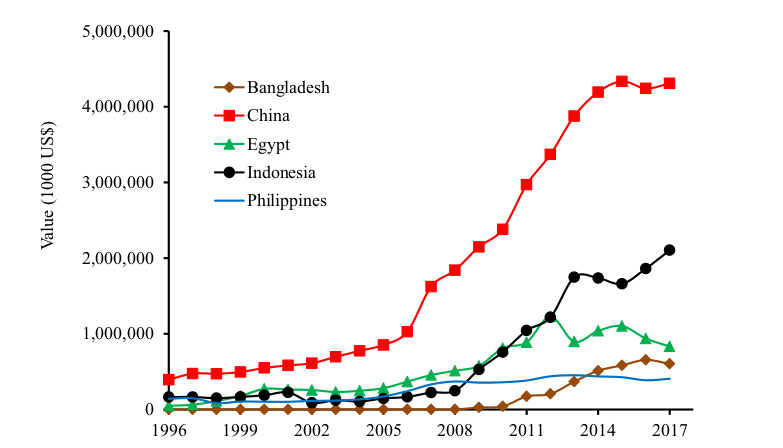
\includegraphics[keepaspectratio, width=12cm]{gambar/produksi_nila}
	\caption{Produksi \emph{Tilapia} 1996-2017 (Fattah, 2020)}
	\label{gambar:produksi_nila}
\end{figure}

Diantara jenis ikan air tawar yang memiliki nilai ekonomi, Lele dan Nila adalah jenis ikan yang memiliki masa panen yang cenderung singkat. Masing-masing memiliki masa panen 3 bulan serta 5 bulan. Ikan Nila (\textit{Tilapia}) memegang 8 persen dari total produksi ikan dunia dengan produksi meningkat dari tahun ke tahun \citep{fattah2020}, hal tersebut dapat dilihat pada gambar 1.1. Sementara itu data KKP menunjukkan, volume produksi \textit{Tilapia} di pulau jawa juga memiliki tren yang sama. Kecuali DKI Jakarta yang stagnant dan Jawa Barat yang menurun, seperti yang ditunjukan oleh gambar 1.2. DKI Jakarta tidak memiliki lahan pertanian yang tidak luas sehingga dapat dimaklumi, untuk Jawa Barat penyebab penurunnya masih perlu dihuhungkan dengan ekspor-impor \textit{Tilapia}, dan jumlah pertumbuhan rumah tangga perikanan \citep{kkp2022}. Ditinjau dari gambar 1.3, indeks konsumsi ikan di Jawa Barat trendnya mengalami peningkatan sehingga logika yang wajar dari turunnya jumlah produksi ikan di Jawa Barat adalah tidak terupdatenya data.

\begin{figure}[H]
	\centering
	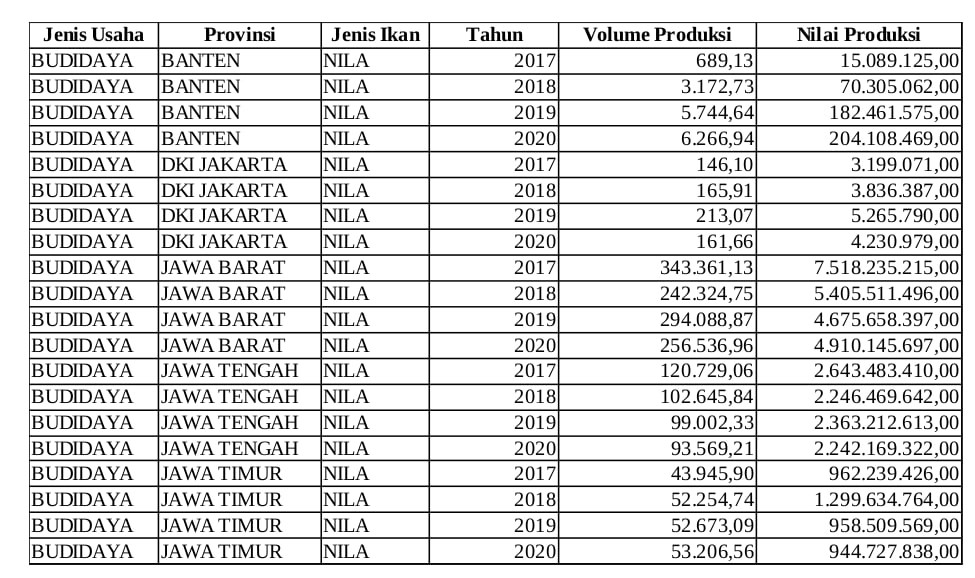
\includegraphics[keepaspectratio, width=13cm]{gambar/produksi_tilapia_jawa}
	\caption{Produksi \emph{Tilapia} Di Pulau Jawa (KKP, 2021)}
	\label{gambar:produksi_tilapia_jawa}
\end{figure}
\begin{figure}[H]
	\centering
	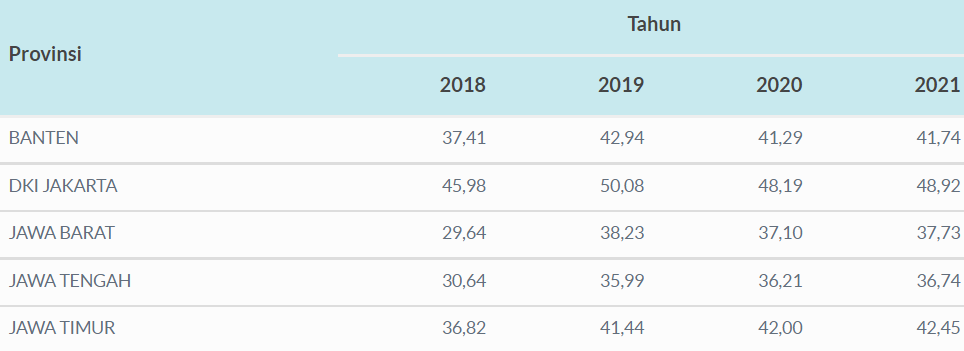
\includegraphics[keepaspectratio, width=12cm]{gambar/indeks_konsumsi_ikan2}
	\caption{Indeks Konsumsi Ikan Di Pulau Jawa (KKP, 2022)}
	\label{gambar:indeks_konsumsi_ikan2}
\end{figure}

Budidaya ikan air tawar di Indonesia secara umum terbagi menjadi 3 kelas yaitu \textit{extensive}, \textit{Semi-Intensive} dan \textit{Intensive}. Budidaya ekstensif adalah budidaya yang dilakukan dengan alami tanpa ada penambahan pakan buatan dari kata tradisional atau ekstensif seharusnya kita mengerti apa itu tradisional. Sementara untuk intensif dan semi-intensif, perbedaan dari keduanya terdapat pada kemampuan tebar padat ikan, dimana \textit{Intensive aquaculture system} mampu mengakomodasi kepadatan ikan dengan luas penampang lahan yang sama. \textit{Semi Intensive} salah satu contohnya pada sistem Tambak. Sementara \textit{Intensive system} diwakili oleh \textit{Biofloc Technology (BFT)} dan \textit{Recirculating Aquaculture System (RAS)}. Ditinjau dari tingkat keahlian yang dibutuhkan \textit{BFT} memerlukan tenaga ahli khusus. 

Kualitas air yang dihasilkan pada \textit{BFT} di atas kualitas air biasa terutama dalam 2 hal yakni, kekayaan dari bahan organik dalam air, dan kemamuan air dalam mereduksi \textit{toxic} secara alami. \textit{BFT} mendapatkan hal tersebut dengan bantuan \textit{Microbacteria} dari keluarga \textit{Bacillus sp} \citep{fattah2020}. \textit{RAS} memiliki kelebihan yaitu tidak dibutuhankan teknisi khusus kecuali saat instalasi kolam. Namun, \textit{RAS} memiliki kemampuan tebar padat yang lebih rendah dibanding \textit{BFT} sehingga skala produktivitasnya masih lebih rendah dibanding sistem \textit{BFT}. Sistem \textit{BFT} memiliki kemampuan tebar padat yang tinggi seperti yang di tunjukan pada gambar 1.4. Namun demikian \textit{BFT} memiliki kelemahan utama yaitu butuh tenaga ahli yang mumpuni atau rumah tangga yang mengaplikasikan \textit{BFT} akan mengalami kegagalan. Dari data peningkatan produksi ikan hasil budidaya ikan air tawar yang telah penulis sebutkan diatas, maka penulis tertarik untuk melakukan penelitian terkait budidaya ikan air tawar untuk membantu pembudidaya dalam melakukan kegiatannya.

\begin{figure}[H]
	\centering
	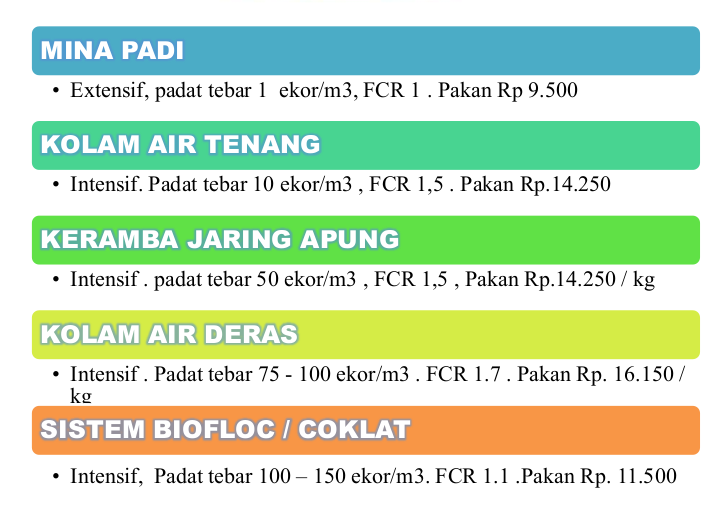
\includegraphics[keepaspectratio, width=9cm]{gambar/tebar_padat}
	\caption{Perbandingan Tebar Padat Kolam \citep{setiawan2021}}
	\label{gambar:tebar_padat}
\end{figure}

Dalam penelitian ini, penulis telah melakukan wawancara dengan UD Jfam sebagai salah satu lembaga budidaya yang bergerak di bidang budidaya ikan air tawar modern berbasis \textit{BFT} yang beralamat di desa Pamagersari, kecamatan Jasinga, Kabupaten Bogor yang menjadi narasumber. Narasumber mengungkapkan permasalahan yang dihadapi selama proses budiddaya di antarnya tenaga ahli bidang \textit{BFT} di UD Jfarm melakukan pemeriksaan kualitas air yang ketat setiap hari. Pengukuran kualitas air ini dilakukan untuk setiap kolam budidaya yang ada seperti yang ditunjukkan pada Gambar 1.5. Hal ini tentunya berimplikasi pada pengelolaan arsip formulir tersebut perlu dilakukan dengan benar dan rapi agar data yang dikumpulkan dapat dievaluasi sebagai dasar pertimbangan \textit{treatment} yang akan dilakukan pada suatu kolam budidaya. Jika hal ini tidak dilakukan, maka berpotensi pada kegagalan proses budidaya berbasis \textit{BFT}. Potensi kegagalan tersebut juga diperbesar dengan metode pencatatan yang dilakukan masih berbasis kertas. Atas dasar masalah tersebut, penulis mengusulkan pengembangan aplikasi pendukung teknologi perikanan modern yang dapat membantu pembudidaya ikan air tawar, dalam hal ini UD Jfam melakukan pencatatan data yang dibutuhkan selama musim budidaya berlangsung.

\begin{figure}[H]
	\centering
	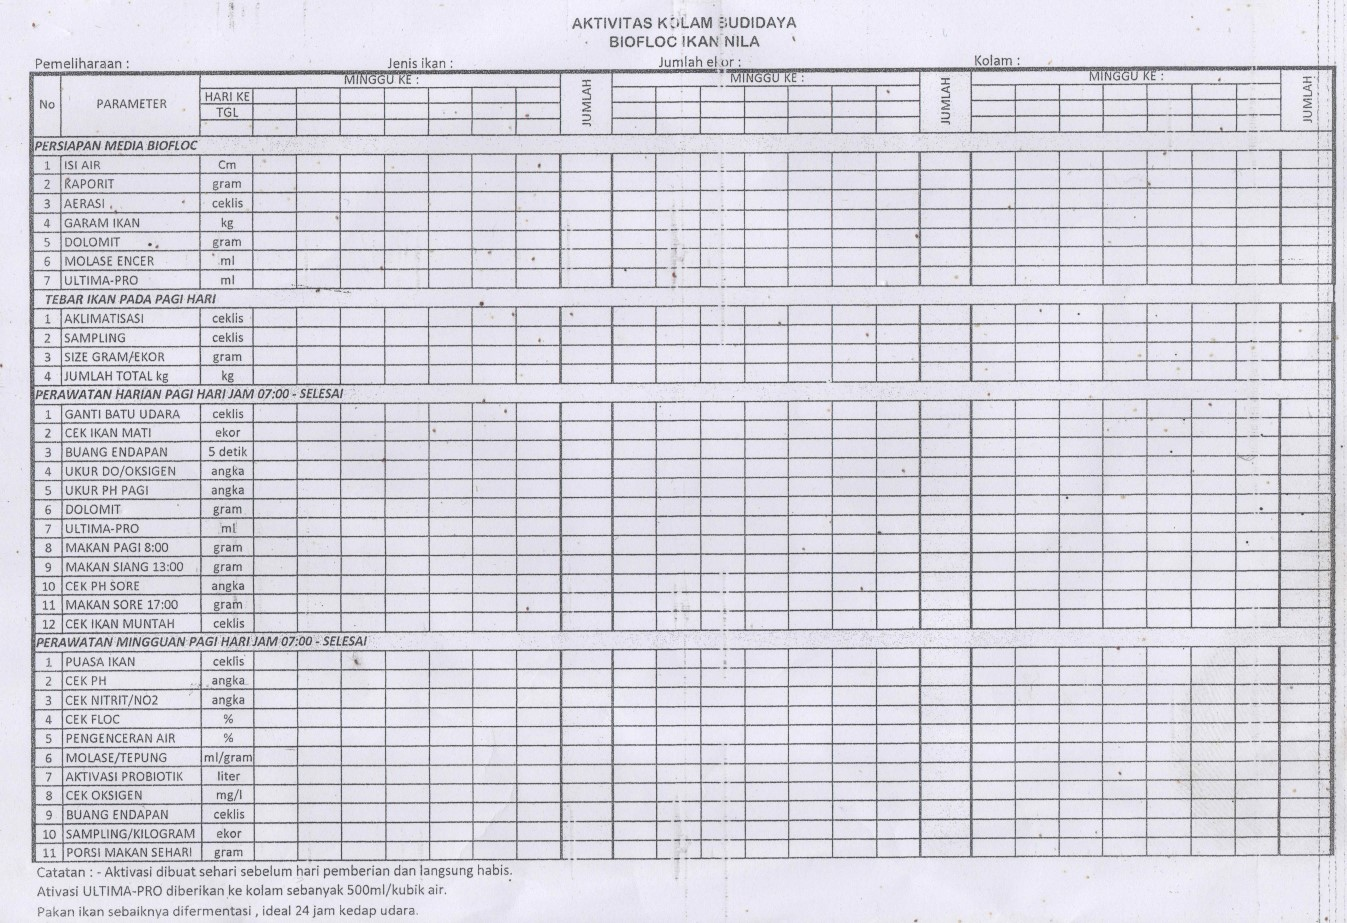
\includegraphics[keepaspectratio, width=14cm]{gambar/form_pencatatan_manual}
	\caption{Form Pencatatan Kualitas Air}
	\label{gambar:form_pencatatan_manual}
\end{figure}

Sudah banyak peneliti di Indonesia  yang berkontribusi dalam berbagai teknologi \textit{Aqua Culture}. \citep{supriati2018} meneliti dan mengembangkan Sistem Informasi Akuntansi Budidaya Perikanan berbasis \textit{SAK EMKM} dan \textit{Android}. Aplikasi yang dikembangkan diperuntukkan untuk Kelompok Tani yang tersusun atas Ketua, Sekretaris, Bendahara, dan Seksi Sarana Produksi perikanan. Aplikasi ini memfasilitasi sejumlah fitur seperti transaksi jual-beli, kas keluar-masuk, dan pembukuan. Penelitian yang sejenis dilakukan oleh \citep{widhiastika2021}, aplikasi hasil penelitian memfasilitasi user untuk melakukan transaksi jual beli perikanan. Aplikasi yang dibuat dinamakan dengan FO-KLIK. Dikembangkan dengan \textit{Android} yang dipasangkan dengan \textit{Firebase}. Selain transaksi jual beli, FO-Klik turut menyediakan fasilitas diskusi dan informasi nilai gizi dari suatu produk item perikanan. Namun tidak dilengkapi dengan manajemen keuangan seperti yang dilakukan oleh \citep{supriati2018}. Selain dari penelitian diatas, perancangan aplikasi terkait budidaya ikan air tawar juga dapat dilakukan berdasarkan metode atau sistem budidaya yang digunakan. Adapun skripsi Andri Rahmanto yang berjudul "Perancangan Arsitektur Aplikasi Budidaya Perikanan Modern pada \textit{Backend} yang Bertanggung Jawab Melayani Transaksi \textit{Query Webservice} Dengan Menggunakan Teknologi \textit{Flask Microservice}" dimana penulis akan menggunakan \textit{Backend} yang telah buat dalam bentuk \textit{REST API}.

Berdasarkan latar belakang yang telah dijelaskan, Peneliti mengusulkan pengembangan aplikasi manajemen budidaya perikanan. Aplikasi ini berpotensi meningkatkan jumlah ikan yang dipanen dan menurunkan angka kematian sehingga mampu menurunkan harga jual ikan dengan adanya stok melimpah. Dengan demikian, dapat terwujud ketahanan pangan wilayah. Aplikasi ini diharapkan dapat membantu petani meningkatkan efisiensi dari setiap masa budidaya yang dijalani.

\section{Rumusan Masalah}
Dari uraian latar belakang di atas, perumusan masalah pada penelitian ini ialah “Bagaimana perancangan aplikasi pendukung teknologi perikanan modern berbasis android?”

\section{Pembatasan Masalah}
Pembatasan masalah pada penelitian ini yaitu:
\begin{enumerate}
	\item Aplikasi pendukung teknologi perikanan modern dikembangkan sampai pada fitur pencatatan dan manajemen masa budidaya.
		
	\item Penelitian ini hanya merangcang bagian \textit{frontend} dari aplikasi pendukung teknologi perikanan modern	 			
\end{enumerate}

\section{Tujuan Penelitian}

 Membuat aplikasi pendukung teknologi perkanan modern yang memudahkan pencatatan data budidaya perikanan.

\section{Manfaat Penelitian}
\begin{enumerate}
	\item Bagi penulis
		
	Memperluas pengetahuan tentang teknologi perikanan modern, menambah pengalaman dalam \textit{programming}, memperoleh gelar sarjana di bidang Ilmu Komputer, serta menjadi media untuk penulis dalam mengaplikasikan ilmu yang didapatkan dari kampus.
		
	\item Bagi Program Studi Ilmu Komputer
	 	
	Penelitian ini dapat menjadi pembuka untuk penelitian di masa depan, dan dapat memberikan panduan bagi mahasiswa program studi Ilmu Komputer tentang perancangan aplikasi teknologi perikanan modern.
	
	\item Bagi Universitas Negeri Jakarta
	 	
	Menjadi evaluasi akademik program studi Ilmu Komputer dalam penyusunan skripsi sehingga dapat meningkatkan kualitas pendidikan dan lulusan program studi Ilmu Komputer di Universitas Negeri Jakarta.
	 			
\end{enumerate}


% Baris ini digunakan untuk membantu dalam melakukan sitasi
% Karena diapit dengan comment, maka baris ini akan diabaikan
% oleh compiler LaTeX.
\begin{comment}
\bibliography{daftar-pustaka}
\end{comment}
